%Encabezado estándar
\documentclass[10pt,a4paper]{article}
\usepackage{pgfplots}
\usepackage[utf8]{inputenc}
\usepackage{amsmath}
\usepackage{multirow}
\usepackage{amssymb}
\usepackage{amsthm}
\usepackage{hyperref}
\usepackage{graphicx}
\usepackage{subfigure} %paquete para poder añadir subfiguras a una figura
\usepackage{listings}
\usepackage{color}
\usepackage{float}
\usepackage[toc,page]{appendix} %paquete para hacer apéndices
\usepackage{cite} %paquete para que Latex contraiga las referencias [1-4] en lugar de [1][2][3][4]
\usepackage[nonumberlist]{glossaries} %[toc,style=altlistgroup,hyperfirst=false] 
%usar makeglossaries grafo para recompilar el archivo donde están los grafos y que así salga actualizado
\author{Gustavo Rivas Gervilla DNI: 75570417F \\ gustavofox92@correo.ugr.es \\5º Doble Grado en Ing. Informática y Matemáticas \\Grupo 3}
\title{Práctica 5.b: Búsquedas Híbridas para el Problema de la Selección de Características \\ AM-(10,1.0) \\ AM-(10,0.1) \\ AM-(10,0.1mej)}
\date{}

\addtolength{\oddsidemargin}{-.875in}
\addtolength{\evensidemargin}{-.875in}
\addtolength{\textwidth}{1.55in}
%Configuración especial
\setlength{\parindent}{0cm}
\pretolerance=10000
\tolerance=10000
\renewcommand{\contentsname}{\color[rgb]{0.0,0.0,0.21}Índice}
\renewcommand{\tablename}{\color[rgb]{0.5,0.0,0.0}Tabla}

\hypersetup{
  colorlinks=true,%colorear el texto en lugar de poner una caja de color alrededor
  citecolor=orange,%citas bibliográficas, del estilo [8]
  urlcolor=orange,%urls
  linkcolor=[rgb]{0.0,0.0,0.21}}%links internos como los del índice
  
\lstdefinestyle{customPy}{
  belowcaptionskip=1\baselineskip,
  breaklines=true,
  frame=L,
  xleftmargin=\parindent,
  language=Python,
  showstringspaces=true,
  basicstyle=\footnotesize\ttfamily,
  keywordstyle=\bfseries\color{green!40!black},
  commentstyle=\itshape\color{purple!40!black},
  identifierstyle=\color{blue},
  stringstyle=\color{orange},
}

\begin{document}
\lstset{language=Python, style=customPy}
\maketitle

\newpage

\tableofcontents

\newpage

\section{\color[rgb]{0.0,0.0,0.21}Descripción/formulación del problema abordado}
Lo que intentamos hacer con nuestros algoritmos es encontrar un conjunto de características de unos datos que nos permitan realizar una clasificación suficientemente buena de nuevos datos que nos lleguen con las mismas características.\\

Hay un problema muy habitual en la vida real y es la de clasificar una serie de elementos en distintas categorías en función de información sobre ellos, esta tarea puede ser realizada por personas o, lo que es más eficiente, por un ordenador. Para realizar tal clasificación es habitual que se recojan multitud de datos sobre los distintos elementos que se quieren clasificar, de modo que en base a esta información podamos decidir si el elemento es de una categoría o de otra. Pensemos por ejemplo en clasificar fruta en base a si se desecha o no. Podemos pensar en recoger datos sobre el tamaño de esa fruta, su color, su textura o su dureza y en base a estas mediciones una máquina debería clasificar la fruta en buena o mala.\\

El problema está en que normalmente no se conoce tan bien el campo de estudio como para saber a ciencia cierta qué datos recoger, qué datos serán más relevantes a la hora de clasificar elementos de una determinada población. Entonces lo que se hace es recoger gran cantidad de información sobre los elementos para al menos intentar que no haya carencias en la información, esto por supuesto conlleva tanto el coste de adquirir esa información (no sabemos cómo de caro es realizar una determinada medición) como el coste computacional de procesar toda esa información. Entonces lo que nos gustaría es averiguar qué información, de entre toda la que hemos obtenido, es la verdaderamente relevante para la clasificación que queremos realizar.\\

Entonces partiendo de un conjunto de datos de aprendizaje, valores de características de distintos elementos, queremos ver con qué subconjunto de características podemos hacer una buena clasificación de esos elementos, así si tenemos que cada dato viene dado por una lista de n características $[f_1, f_2, ..., f_n]$ queremos obtener un subconjunto de esas características, de modo que teniendo sólo la información $[f_{s1}, ..., f_{sm}]$, se haga una buena clasificación del conjunto de datos de aprendizaje, del que conocemos por supuesto la clasificación perfecta de dichos datos. Y esperamos que con esa misma información se clasifiquen lo mejor posible nuevos elementos de fuera de la muestra de aprendizaje.\\

\newpage

\section{\color[rgb]{0.0,0.0,0.21}Descripción de la aplicación de los algoritmos empleados al problema}

Dado que estamos ante un problema de selección las soluciones se representarán como vectores binarios de booleanos de tamaño el número de características a elegir, indicando si una característica se considera o no, así tendremos claramente un espacio de búsqueda de $2^n$, siendo $n$ el número de características a elegir que también lo podemos ver como el tamaño del problema abordado.\\

Entonces para evaluar como de buena es una determinada solución hacemos lo siguiente, que es nuestr función objetivo:\\

\begin{lstlisting}
tomamos de cada dato de entrenamiento las caracteristicas seleccionada por la solucion.

for cada dato de entrenamiento:
	clasificador_dato = construir clasificador 3NN con el resto de datos
	ver si clasificador_dato clasifica correctamente a ese dato
	
return porcentaje de aciertos
\end{lstlisting}

Nuestros algoritmos irán explorando, según su mecanismo, el espacio de soluciones empleando la función anterior para tomar decisiones sobre qué movimientos se realizan en dicho espacio de búsqueda. Para poder generar las soluciones vecinas a una dada empleamos el operador de Flip, el cual funciona del siguiente modo:\\

\begin{lstlisting}
def flip(sol, idx):
	cambiar el valor de la pos. idx de la sol por su negado
\end{lstlisting}

Cuando finalice su proceso de búsqueda los algoritmos nos devolverán la solución que ellos han elegido (junto con el score dentro de la muestra de entrenamiento calculada como hemos dicho antes). Entonces una vez tenemos la solución nos queda por evaluar cómo de bien se clasifican los datos empleando un clasificador 3NN construido sólo con aquellas características seleccionadas por nuestra solución:\\

\begin{lstlisting}
claficador = construir clasificador con los datos de entrenamiento solo con las caracterisiticas seleccionadas por nuestra solucion
return el porcentaje de acierto de este clasificador etiquetando los datos de test de los que consideramos solo las caracteristicas seleccionadas por la solucion
\end{lstlisting}

A cada algoritmo le daremos solamente los datos de entrenamiento separados en características y etiquetas pera que con la estragia de búsqueda que implemente nos devuelva la mejor solución posible para él, luego la evaluación de la solución final la haremos fuera del algoritmo con los datos de test (en la sección 8 explicaremos cómo hemos generado las particiones). Para aquellos algoritmos que empleando algún tipo de aleatoriedad en sus decisiones inicilizaremos la semilla aleatoria antes de la ejecución de dicho algoritmo.\\

Para generar las soluciones aleatorias lo que hacemos al inicio de cada algoritmo es:\\

\begin{lstlisting}
p_inicial = vector[30][num_caracteristicas]

for cada p in p_inicial:
	p = vector de num_caracteristicas valores booleanos aleatorios
\end{lstlisting}

El mecanismo de BL que vamos a emplear para hibridar con el AGG es el mismo algoritmo que implementamos en la Práctica 1 pero realizando sólamente una iteración, antes repetíamos el proceso de búsqueda local si en la iteración anterior habíamos encontrado una solución mejor, ahora la BL es como sigue:\\

\begin{lstlisting}
s = individuo a optimizar que le pasamos

for cada vecino de s explorados en orden aleatorio mientras no se encuentre otro mejor
o no acabemos la exploracion:
	
		if el vecino es mejor que s:
			s = el vecino		
			
return s, s_score, evaluacionesDeObjetivo
\end{lstlisting}

\newpage

\section{\color[rgb]{0.0,0.0,0.21}Descripción en pseudocódigo de los algoritmos}

Todos los algoritmos están implementados en el fichero \textbf{AM.py} donde la función AM recibe como argumento qué modelo de optimización de soluciones emplear y en base a ese modelo aplica el mecanismo de BL a unos individuos de la poblacion u otros. Así divideremos la descripción en pseudocódigo en dos partes, la parte evolutiva común a todos los modelos y la parte de optimización distinta para cada uno:\\

\subsection{\color[rgb]{0.0,0.0,0.51} Parte evolutiva común}

\begin{lstlisting}
padres = poblacion inicial de 30 individuos aleatoria
ordenamos los padres de peor a mejor segun score
n_evals += 30
n_generaciones = 0

while n_evals < max_evals:
	n_generaciones++
	#seleccion
	padres_seleccionados = seleccionamos 30 padres por torneo binario (con repeticion)
	
	#cruce
	cruzamos las primeras n_cruces parejas de padres_seleccionados y metemos el resultado en hijos
	
	aniadimos a hijos copias de los padres que no se han cruzado
	
	n_evals += 2*n_cruces
	
	#mutacion
	seleccionamos n_mutaciones hijos aleatoriamente para mutar (con repeticion)
	seleccionamos n_mutaciones genes a mutar (con repeticion)
	
	for cada par (hijo,gen) seleccionado:
		modificamos el gen de ese hijo por su complementario
		
	n_evals += n_mutaciones
		
	#remplazamiento
	if mejor_hijo es peor que mejor_padre:
		peor_hijo = mejor_padre
		
	padres = hijos
	ordenamos padres
	
	if n_generaciones == 10:
		n_generaciones = 0
		mecanismo de optimizacion correspondiente
		n_evals += numero evaluaciones empleados en el proceso de optimizacion
	
return mejor padre de la poblacion actual		
\end{lstlisting}

\newpage

\subsection{\color[rgb]{0.0,0.0,0.51}Mecanismo de optimización AM-(10,1.0)}

\begin{lstlisting}
for cada padre:
	padre = BL1iteracion(sol. inicial = padre)
\end{lstlisting}

\subsection{\color[rgb]{0.0,0.0,0.51}Mecanismo de optimización AM-(10,0.1)}

Aquí empleamos que el tamaño de nuestra población es 10 y en consecuencia, para no generar 10 números, lo que hacemos es, dado que la probabilidad es 0.1, optimizar un individuo al azar:\\

\begin{lstlisting}
padre = padre aleatorio elegido entre los padres
padre = BL1iteracion(sol. inicial = padre)
\end{lstlisting}
\subsection{\color[rgb]{0.0,0.0,0.51}Mecanismo de optimización AM-(10,0.1mejor)}

Como la población es de tamaño 10 entonces se optimizará solamente al mejor de la población de padres:\\

\begin{lstlisting}
mejor_padre = BL1iteracion(sol. inicial = mejor_padre)
\end{lstlisting}

\newpage

\section{\color[rgb]{0.0,0.0,0.21}Breve descripción del algoritmo de comparación}

Para el algoritmo de comparación, SFS, lo que hacemos es lo que vamos a reflejar en el siguiente pseudocódigo, la principal diferencia es que no tenemos la función usual flip sino que hemos hecho una función especial para poder realizar una función vectorizada en Python (aunque no produce ninguna mejora en tiempo a la versión que tendríamos si simplemente tuviésemos un for que recorriese las características que quedan por añadir hasta encontra la de mayor ganancia), esta función crea una nueva solución poniendo a True una componente de la solución que le pasamos y nos da su porcentaje de clasificación, como hacemos en el resto de algoritmos. Dicho esto pasamos al pseudocódigo:

\begin{lstlisting}
sol = un array binario con todo False #conjunto vacio de caracteristicas

while tengamos ganancia and queden caracteristicas por aniadir:
	calcular el score de cada caracteristica por aniadir al agregarla al conjunto actual
	tomar la caracteristica que de mejor score en el calculo anterior
	
	if el score aniadiendola es mejor que el de el conjunto mejor al que habia:
		se agrega dicha caracteristica al conjunto
		quitamos esa caracteristica de el conjunto de caracteristicas por aniadir
	else:
		no tenemos ganancia y acabamos el bucle
		
return el conjunto de caracteristicas al que hemos llegado
\end{lstlisting}
\newpage

\section{\color[rgb]{0.0,0.0,0.21}Procedimiento considerado para desarrollar la práctica}

\subsection{\color[rgb]{0.0,0.0,0.51}Desarrollo}

El código usado en prácticas lo he implementado yo a partir de las explicaciones dadas tanto en clase de prácticas como de teoría sobre los distintos algoritmos, siendo de mucha utilidad las indicaciones del gruión de práctias y del seminario.\\

La parte que no ha sido implementada por mí es la correspondiente a la evaluación de las soluciones, es decir, tanto el KNN como los mecanismos de evaluación de las soluciones. Para ello he usado el código desarrollado por \textbf{Alejandro García Montoro} el cuál ha implementado tanto el clasificador KNN como los mecanismos para obtener el score de las soluciones dentro (con LOO) y fuera de la muestra con PyCUDA que permite insertar código CUDA en código Python. Con lo cual los tiempos de ejecución bajan considerablemente con respecto a los tiempos de la práctica anterior ya que el cuello de botella de los algoritmos, que es la evaluación de las soluciones con LOO, se ejecuta en la tarjeta gráfica, siendo mucho más rápidos los cálculos.\\

\subsection{\color[rgb]{0.0,0.0,0.51}Manual de usuario}
Los algoritmos han sido implementados en Python 3.5.1 para su ejecución son necesarios tener instalados los módulos compatibles con esta versión de Python siguientes:\\

\begin{itemize}
\item numpy (v 1.8.2) \textbf{sudo apt-get install python-numpy}
\item scikit \textbf{sudo apt-get install python-scikits-learn}
\item jinja2
\item pycuda
\item El resto de módulos empleados suelen venir con las distribuciones básicas de Python (random, sys y time).
\end{itemize}

Cada uno de los algoritmos están implementados en distintos ficheros de los que podemos ver su contenido en el \textbf{\textcolor{green}{LEEME}} que se nos pide que incluyamos con el código. Los experimentos han sido ejecutados usando el fichero main al que le pasamos por argumentos el nombre del algoritmo a usar: 3NN, SFS, AGG o AGE. La semilla se establece dentro del fichero al inicio de la ejecución del algoritmo para cada una de las particiones. Esto lo hemos hecho así para poder cortar la obtención de datos cuando sea necesaria y poder retomar los experimento desde la partición por las que nos quedáramos, así no se desajusta la semilla con la que hacemos los experimentos al retomar.\\

Entonces para ejecutar por ejemplo los experimentos para el AGG lo que haremos es \textit{python mainCUDA.py AGG} y se ejecutará el algoritmo sobre todas las particiones de datos que tenemos.\\

En el directorio \textbf{\textcolor{green}{make\_partitions32b}} tenemos tanto los archivos arff como los códigos necesarios para elaborar las particiones que serán utilizadas por nuestros algoritmos. Esto no es necesario para ejecutar los programas puesto que en el directorio \textbf{\textcolor{green}{partitions32b}} tenemos almacenadas todas las particiones construidas. No obstante si se quisiera replicar el procedimiento de desarrollo de particiones lo que haríamos sería: eliminar los archivos con extensión .npy del directorio \textbf{make\_partitions32b} (para tener seguridad de que no se corrompan dichos archivos), ejecutar el loader con la instrucción \textbf{python loader.py} y a continuación elaborar las particiones con \textbf{python partition\_maker.py} (dentro de este directorio que es donde se encuentran ambos códigos). Esto generará diversos archivos de extensión .npy con nombres que empiezan por arr, wdbc o libras (según la base) seguida de un número y la palabra test o training.\\

Estos archivos deberán reemplazar a aquellos que se encuentran en el directorio \textbf{partitions32b} y ya podremos ejecutar los algoritmos con dichas particiones desde el main.\\

\newpage
\section{\color[rgb]{0.0,0.0,0.21}Experimentos y análisis de resultados}

\subsection{\color[rgb]{0.0,0.0,0.51}Descripción de los casos del problema empleados y de los valores de los parámetros}


Estás prácticas han sido implementadas en Python 3.5.1 y ejecutadas sobre un ordenador son S.O. Arch Linux, de 12GB de RAM y procesador Intel Core i7 930 2.80GHz y tarjeta gráfica NVIDIA GeForce GTX 780. Este ordenador pertenece a Alejandro Garcia Montoro ya que tuve problemas al intentar usar los drivers oficiales de Nvidia en Ubuntu (necesarios para ejecutar código CUDA) y me ha permitido lanzar mis códigos en su ordenador mediante conexión ssh.\\

Hemos empleado tres bases de datos distintas, a continuación mencionamos sus tamaños ya pueden ser interesantes para el posterior análisis de resultados:\\

\begin{itemize}
\item \textbf{wdbc}: Tenemos \textbf{569} muestras con \textbf{30} características cada una procedentes de imágenes digitalizadas de una masa de mama. Estas muestras se clasifican en \textbf{2} clases distintas.
\item \textbf{libras}: Aquí tenemos \textbf{360} muestras de \textbf{90} características cada una, éstas muestras son datos de distintos movimientos de la mano que se clasifican en \textbf{15} clases distintas.
\item \textbf{arritmia}: Los datos de este conjunto son mediciones para determinar la presencia de arritmia cardiaca o no. Tenemos \textbf{386} muestras con \textbf{278} caracterísitcas cada una, a clasificar en \textbf{5} grupos en base al tipo de arritmia que indican los datos de la muestra.
\end{itemize}

Lo que hemos hecho con los datos ha sido un preprocesado, en primer lugar todos los datos han sido codificados como flotantes (las etiquetas de wdbc eran cadenas de texto y las hemos cambiado por los valores 0 y 1), también hemos puesto la etiqueta en la última columna de la tabla de datos. Es importante señalar que para poder emplear el KNN implementado en pyCUDA que hemos mencionado antes hemos tenido que codificar los distintos datos de las particiones en 32 bits ya que así es como estaba configurado el clasificador y CUDA no hace correctamente el casting de 64b a 32b.\\

También hemos normalizado cada una de las columnas de datos (sin contar la de etiquetas) de modo que los valores quedaran en el intervalo [0,1] mediantes la fórmula:\\

\begin{center}
$x_j^N = \dfrac{x_j - Min_j}{Max_j-Min_j}$ (siendo $Max_j$ y $Min_j$ el máximo y mínimo valor de los datos para la característica j-ésima de las muestras).
\end{center}

El código empleado para este formateo de los datos está en el fichero \textbf{\textcolor{green}{loader.py}} que se adjunta en la entrega. Como podemos ver para realizar la normalización de los datos hemos usado una utilidad del módulo scikit-learn antes mencionado que se llama MinMaxScaler. Y para futuros usos de estos datos normalizados, y con el objetivo de no tener que realizar tales operaciones cada ocasión que queramos usarlos, hemos almacenado los arrays de numpy donde hemos almacenado los datos en sendos ficheros con extensión .npy usando la función \textbf{numpy.save}. Estos ficheros son: \textbf{\textcolor{green}{data\_wdbc.npy}}, \textbf{\textcolor{green}{data\_libras.npy}} y \textbf{\textcolor{green}{data\_arrhythmia.npy}}.\\

A continuación hemos elaborado las distintas particiones sobre estos datos que serán utilizadas en los experimentos, para ello hemos elaborado el código recogido en el fichero \textbf{\textcolor{green}{partition\_maker.npy}} donde simplemente tomamos una muestra aleatoria de los índices de los arrays antes generados, teniendo en cuenta que la cantidad de muestras de cada una de las clases en las que se clasifican los datos sea lo más equilibrida posible entre la partición de test y su correspondiente partición de training. La semilla usada para la generación de dichas particiones, y que podemos ver en el fichero mencionado, ha sido la \textbf{12345678}. Nuevamente hemos almacenado cada una de dichas particiones en ficheros .npy, los cuáles están en la carpeta \textbf{\textcolor{green}{partitions32b}}.\\

Los parámetros empleados en cada uno de los algoritmos son los que se indican en el guión de prácticas. Para cada una de las ejecuciones de lo algoritmos inicializamos la semilla aleatoria a \textbf{12345678} nuevamente, esto lo podemos ver en el fichero \textbf{\textcolor{green}{mainCUDA.py}}.\\


\subsection{\color[rgb]{0.0,0.0,0.51}Resultados}

Adjuntamos también las tablas en un fichero por si no se leen correctamente en el pdf.

% Please add the following required packages to your document preamble:
% \usepackage{multirow}
\begin{table}[H]
\centering
\caption{3NN}
\label{my-label}
\resizebox{\textwidth}{!}{\begin{tabular}{l|l|l|l|l|l|l|l|l|l|l|l|l|}
\cline{2-13}
\multirow{2}{*}{}                   & \multicolumn{4}{c|}{Wdbc}                     & \multicolumn{4}{c|}{Movement\_Libras}         & \multicolumn{4}{c|}{Arrhythmia}               \\ \cline{2-13} 
                                    & \%\_clas\_in & \%\_clas\_out & \%\_red & T    & \%\_clas\_in & \%\_clas\_out & \%\_red & T    & \%\_clas\_in & \%\_clas\_out & \%\_red & T    \\ \hline
\multicolumn{1}{|l|}{Partición 1-1} & 96,14        & 96,13         & 0,00    & 0,00 & 75,56        & 76,11         & 0,00    & 0,00 & 65,46        & 64,06         & 0,00    & 0,00 \\ \hline
\multicolumn{1}{|l|}{Partición 1-2} & 96,83        & 95,79         & 0,00    & 0,00 & 67,78        & 70,56         & 0,00    & 0,00 & 59,38        & 62,37         & 0,00    & 0,00 \\ \hline
\multicolumn{1}{|l|}{Partición 2-1} & 95,44        & 96,47         & 0,00    & 0,00 & 70,00        & 67,78         & 0,00    & 0,00 & 62,89        & 62,50         & 0,00    & 0,00 \\ \hline
\multicolumn{1}{|l|}{Partición 2-2} & 96,13        & 96,49         & 0,00    & 0,00 & 74,44        & 72,78         & 0,00    & 0,00 & 63,02        & 64,43         & 0,00    & 0,00 \\ \hline
\multicolumn{1}{|l|}{Partición 3-1} & 93,68        & 97,18         & 0,00    & 0,00 & 70,56        & 73,33         & 0,00    & 0,00 & 60,82        & 65,10         & 0,00    & 0,00 \\ \hline
\multicolumn{1}{|l|}{Partición 3-2} & 97,54        & 95,44         & 0,00    & 0,00 & 70,00        & 72,22         & 0,00    & 0,00 & 61,98        & 64,95         & 0,00    & 0,00 \\ \hline
\multicolumn{1}{|l|}{Partición 4-1} & 96,14        & 95,42         & 0,00    & 0,00 & 72,22        & 72,22         & 0,00    & 0,00 & 60,82        & 64,58         & 0,00    & 0,00 \\ \hline
\multicolumn{1}{|l|}{Partición 4-2} & 98,24        & 95,44         & 0,00    & 0,00 & 70,00        & 74,44         & 0,00    & 0,00 & 64,58        & 62,37         & 0,00    & 0,00 \\ \hline
\multicolumn{1}{|l|}{Partición 5-1} & 96,14        & 95,42         & 0,00    & 0,00 & 71,11        & 78,33         & 0,00    & 0,00 & 67,01        & 63,02         & 0,00    & 0,00 \\ \hline
\multicolumn{1}{|l|}{Partición 5-2} & 97,89        & 95,44         & 0,00    & 0,00 & 71,67        & 73,33         & 0,00    & 0,00 & 63,54        & 62,37         & 0,00    & 0,00 \\ \hline
\multicolumn{1}{|l|}{Media}         & 96,42        & 95,92         & 0,00    & 0,00 & 71,33        & 73,11         & 0,00    & 0,00 & 62,95        & 63,58         & 0,00    & 0,00 \\ \hline
\end{tabular}}
\end{table}

% Please add the following required packages to your document preamble:
% \usepackage{multirow}
\begin{table}[H]
\centering
\caption{SFS}
\label{my-label}
\resizebox{\textwidth}{!}{\begin{tabular}{l|l|l|l|l|l|l|l|l|l|l|l|l|}
\cline{2-13}
\multirow{2}{*}{}                   & \multicolumn{4}{c|}{Wdbc}                     & \multicolumn{4}{c|}{Movement\_Libras}         & \multicolumn{4}{c|}{Arrhythmia}               \\ \cline{2-13} 
                                    & \%\_clas\_in & \%\_clas\_out & \%\_red & T    & \%\_clas\_in & \%\_clas\_out & \%\_red & T    & \%\_clas\_in & \%\_clas\_out & \%\_red & T    \\ \hline
\multicolumn{1}{|l|}{Partición 1-1} & 95,44        & 95,42         & 83,33   & 0,24 & 78,89        & 72,22         & 90,00   & 1,04 & 79,90        & 68,23         & 97,12   & 3,00 \\ \hline
\multicolumn{1}{|l|}{Partición 1-2} & 97,54        & 92,98         & 90,00   & 0,15 & 74,44        & 60,00         & 93,33   & 0,69 & 74,48        & 70,10         & 98,56   & 1,51 \\ \hline
\multicolumn{1}{|l|}{Partición 2-1} & 97,19        & 97,54         & 86,67   & 0,20 & 77,22        & 66,11         & 88,89   & 1,16 & 84,54        & 71,35         & 97,12   & 3,00 \\ \hline
\multicolumn{1}{|l|}{Partición 2-2} & 97,54        & 95,79         & 90,00   & 0,15 & 76,11        & 65,56         & 91,11   & 0,92 & 72,92        & 69,59         & 99,28   & 0,85 \\ \hline
\multicolumn{1}{|l|}{Partición 3-1} & 96,49        & 95,77         & 83,33   & 0,24 & 78,33        & 73,89         & 90,00   & 1,04 & 77,32        & 69,79         & 97,48   & 2,62 \\ \hline
\multicolumn{1}{|l|}{Partición 3-2} & 97,89        & 95,09         & 86,67   & 0,20 & 76,11        & 75,00         & 91,11   & 0,92 & 85,94        & 74,23         & 96,04   & 4,27 \\ \hline
\multicolumn{1}{|l|}{Partición 4-1} & 95,09        & 91,55         & 93,33   & 0,11 & 76,11        & 67,22         & 91,11   & 0,92 & 79,90        & 67,19         & 96,04   & 4,24 \\ \hline
\multicolumn{1}{|l|}{Partición 4-2} & 98,24        & 94,04         & 76,67   & 0,33 & 70,56        & 65,56         & 93,33   & 0,69 & 83,33        & 78,87         & 96,76   & 3,41 \\ \hline
\multicolumn{1}{|l|}{Partición 5-1} & 96,84        & 97,18         & 86,67   & 0,20 & 68,33        & 62,78         & 93,33   & 0,70 & 84,02        & 69,79         & 96,04   & 4,26 \\ \hline
\multicolumn{1}{|l|}{Partición 5-2} & 98,24        & 94,04         & 83,33   & 0,24 & 74,44        & 66,11         & 92,22   & 0,81 & 83,85        & 73,71         & 96,04   & 4,25 \\ \hline
\multicolumn{1}{|l|}{Media}         & 97,05        & 94,94         & 86,00   & 0,21 & 75,05        & 67,45         & 91,44   & 0,89 & 80,62        & 71,29         & 97,05   & 3,14 \\ \hline
\end{tabular}}
\end{table}

% Please add the following required packages to your document preamble:
% \usepackage{multirow}
\begin{table}[H]
\centering
\caption{BL}
\label{my-label}
\resizebox{\textwidth}{!}{\begin{tabular}{l|l|l|l|l|l|l|l|l|l|l|l|l|}
\cline{2-13}
\multirow{2}{*}{}                   & \multicolumn{4}{c|}{Wdbc}                     & \multicolumn{4}{c|}{Movement\_Libras}         & \multicolumn{4}{c|}{Arrhythmia}               \\ \cline{2-13} 
                                    & \%\_clas\_in & \%\_clas\_out & \%\_red & T    & \%\_clas\_in & \%\_clas\_out & \%\_red & T    & \%\_clas\_in & \%\_clas\_out & \%\_red & T    \\ \hline
\multicolumn{1}{|l|}{Partición 1-1} & 97,89        & 96,13         & 50,00   & 0,25 & 75,56        & 76,11         & 48,89   & 0,49 & 73,20        & 65,63         & 52,16   & 5,62 \\ \hline
\multicolumn{1}{|l|}{Partición 1-2} & 98,24        & 94,77         & 40,00   & 0,19 & 71,67        & 69,44         & 44,44   & 0,73 & 69,27        & 64,95         & 53,60   & 5,31 \\ \hline
\multicolumn{1}{|l|}{Partición 2-1} & 97,89        & 95,77         & 56,67   & 0,22 & 71,11        & 69,44         & 42,22   & 0,48 & 71,13        & 64,06         & 52,88   & 3,42 \\ \hline
\multicolumn{1}{|l|}{Partición 2-2} & 95,77        & 95,09         & 46,67   & 0,09 & 77,22        & 72,22         & 44,44   & 0,62 & 70,31        & 64,95         & 53,96   & 6,63 \\ \hline
\multicolumn{1}{|l|}{Partición 3-1} & 96,49        & 97,54         & 43,33   & 0,19 & 72,78        & 72,22         & 44,44   & 0,35 & 69,59        & 67,19         & 52,88   & 3,62 \\ \hline
\multicolumn{1}{|l|}{Partición 3-2} & 97,89        & 94,04         & 46,67   & 0,11 & 75,00        & 72,22         & 47,78   & 0,52 & 72,92        & 63,92         & 53,60   & 5,10 \\ \hline
\multicolumn{1}{|l|}{Partición 4-1} & 97,54        & 95,07         & 50,00   & 0,18 & 73,33        & 72,22         & 45,56   & 0,33 & 72,68        & 67,71         & 52,88   & 4,85 \\ \hline
\multicolumn{1}{|l|}{Partición 4-2} & 98,24        & 92,63         & 40,00   & 0,14 & 72,78        & 73,33         & 47,78   & 0,52 & 70,31        & 63,92         & 51,80   & 3,57 \\ \hline
\multicolumn{1}{|l|}{Partición 5-1} & 95,14        & 93,66         & 43,33   & 0,13 & 71,67        & 79,44         & 43,33   & 0,40 & 68,56        & 65,63         & 53,24   & 4,33 \\ \hline
\multicolumn{1}{|l|}{Partición 5-2} & 98,59        & 94,39         & 43,33   & 0,24 & 70,00        & 74,44         & 43,33   & 0,34 & 71,88        & 61,34         & 53,60   & 4,43 \\ \hline
\multicolumn{1}{|l|}{Media}         & 97,37        & 94,91         & 46,00   & 0,17 & 73,11        & 73,11         & 45,22   & 0,48 & 70,99        & 64,93         & 53,06   & 4,69 \\ \hline
\end{tabular}}
\end{table}

\begin{table}[H]
\centering
\caption{AGG}
\label{my-label}
\resizebox{\textwidth}{!}{\begin{tabular}{l|l|l|l|l|l|l|l|l|l|l|l|l|}
\cline{2-13}
                                    & \multicolumn{4}{c|}{Wdbc}                      & \multicolumn{4}{c|}{Movement\_Libras}          & \multicolumn{4}{c|}{Arrhythmia}                 \\ \cline{2-13} 
                                    & \%\_clas\_in & \%\_clas\_out & \%\_red & T     & \%\_clas\_in & \%\_clas\_out & \%\_red & T     & \%\_clas\_in & \%\_clas\_out & \%\_red & T      \\ \hline
\multicolumn{1}{|l|}{Partición 1-1} & 97,54        & 96,83         & 33,33   & 40,28 & 80,00        & 77,78         & 37,78   & 50,25 & 75,77        & 66,15         & 21,22   & 160,57 \\ \hline
\multicolumn{1}{|l|}{Partición 1-2} & 98,24        & 94,74         & 40,00   & 37,62 & 77,22        & 70,00         & 47,78   & 45,31 & 74,48        & 64,95         & 12,59   & 219,25 \\ \hline
\multicolumn{1}{|l|}{Partición 2-1} & 98,25        & 95,77         & 26,67   & 41,89 & 78,33        & 66,67         & 38,89   & 48,90 & 77,32        & 60,94         & 28,06   & 149,95 \\ \hline
\multicolumn{1}{|l|}{Partición 2-2} & 98,59        & 95,09         & 60,00   & 32,82 & 81,11        & 72,22         & 42,22   & 48,72 & 73,96        & 68,04         & 22,66   & 194,06 \\ \hline
\multicolumn{1}{|l|}{Partición 3-1} & 96,84        & 98,59         & 33,33   & 39,79 & 78,33        & 71,67         & 34,44   & 51,50 & 73,20        & 65,10         & 21,94   & 158,43 \\ \hline
\multicolumn{1}{|l|}{Partición 3-2} & 98,94        & 95,09         & 23,33   & 42,68 & 77,22        & 72,78         & 36,66   & 51,00 & 72,40        & 63,92         & 16,55   & 212,03 \\ \hline
\multicolumn{1}{|l|}{Partición 4-1} & 97,89        & 96,13         & 23,33   & 42,34 & 79,44        & 71,11         & 45,56   & 46,56 & 76,29        & 68,23         & 29,14   & 148,91 \\ \hline
\multicolumn{1}{|l|}{Partición 4-2} & 98,94        & 94,74         & 33,33   & 40,28 & 77,78        & 74,44         & 56,67   & 40,84 & 74,48        & 63,40         & 13,67   & 213,18 \\ \hline
\multicolumn{1}{|l|}{Partición 5-1} & 98,25        & 95,07         & 26,67   & 40,89 & 77,78        & 76,11         & 46,67   & 46,05 & 73,20        & 66,67         & 24,82   & 155,78 \\ \hline
\multicolumn{1}{|l|}{Partición 5-2} & 99,3         & 95,44         & 13,33   & 45,53 & 80,00        & 73,89         & 47,78   & 46,12 & 75,00        & 64,43         & 29,14   & 175,24 \\ \hline
\multicolumn{1}{|l|}{Media}         & 98,28        & 95,75         & 31,33   & 40,41 & 78,72        & 72,67         & 43,45   & 47,53 & 74,61        & 65,18         & 21,98   & 178,74 \\ \hline
\end{tabular}}
\end{table}

% Please add the following required packages to your document preamble:
% \usepackage{multirow}
\begin{table}[H]
\centering
\caption{AM-(10,1.0)}
\label{my-label}
\resizebox{\textwidth}{!}{\begin{tabular}{l|l|l|l|l|l|l|l|l|l|l|l|l|}
\cline{2-13}
\multirow{2}{*}{}                   & \multicolumn{4}{c|}{Wdbc}                      & \multicolumn{4}{c|}{Movement\_Libras}          & \multicolumn{4}{c|}{Arrhythmia}                 \\ \cline{2-13} 
                                    & \%\_clas\_in & \%\_clas\_out & \%\_red & T     & \%\_clas\_in & \%\_clas\_out & \%\_red & T     & \%\_clas\_in & \%\_clas\_out & \%\_red & T      \\ \hline
\multicolumn{1}{|l|}{Partición 1-1} & 98,25        & 95,07         & 36,67   & 41,35 & 76,67        & 78,33         & 44,44   & 47,97 & 75,77        & 64,06         & 43,17   & 120,57 \\ \hline
\multicolumn{1}{|l|}{Partición 1-2} & 98,59        & 96,49         & 36,67   & 40,79 & 73,33        & 71,67         & 52,22   & 44,75 & 71,35        & 64,95         & 43,88   & 131,88 \\ \hline
\multicolumn{1}{|l|}{Partición 2-1} & 97,89        & 95,42         & 26,67   & 43,82 & 75,56        & 68,89         & 38,89   & 50,08 & 71,65        & 63,02         & 41,37   & 132,17 \\ \hline
\multicolumn{1}{|l|}{Partición 2-2} & 97,89        & 95,09         & 46,67   & 37,55 & 78,89        & 72,22         & 38,89   & 50,67 & 72,40        & 66,49         & 38,50   & 150,49 \\ \hline
\multicolumn{1}{|l|}{Partición 3-1} & 96,14        & 96,48         & 43,33   & 38,62 & 76,67        & 75,56         & 52,22   & 43,26 & 72,16        & 65,10         & 40,29   & 132,24 \\ \hline
\multicolumn{1}{|l|}{Partición 3-2} & 98,94        & 95,44         & 13,33   & 46,42 & 77,78        & 73,33         & 44,44   & 47,92 & 70,83        & 65,47         & 39,93   & 151,50 \\ \hline
\multicolumn{1}{|l|}{Partición 4-1} & 97,89        & 94,37         & 46,67   & 37,48 & 77,78        & 70,00         & 51,11   & 46,06 & 69,59        & 64,58         & 42,45   & 122,46 \\ \hline
\multicolumn{1}{|l|}{Partición 4-2} & 98,94        & 94,74         & 20,00   & 45,16 & 77,22        & 76,67         & 53,33   & 43,49 & 74,48        & 64,43         & 46,40   & 132,22 \\ \hline
\multicolumn{1}{|l|}{Partición 5-1} & 97,89        & 94,37         & 30,00   & 41,83 & 74,44        & 77,78         & 50,00   & 41,78 & 72,16        & 67,71         & 41,01   & 139,81 \\ \hline
\multicolumn{1}{|l|}{Partición 5-2} & 98,59        & 95,44         & 16,67   & 45,81 & 77,78        & 75,00         & 42,22   & 49,07 & 72,40        & 65,46         & 45,68   & 134,47 \\ \hline
\multicolumn{1}{|l|}{Media}         & 98,10        & 95,29         & 31,67   & 41,88 & 76,61        & 73,95         & 46,78   & 46,51 & 72,28        & 65,13         & 42,27   & 134,78 \\ \hline
\end{tabular}}
\end{table}

% Please add the following required packages to your document preamble:
% \usepackage{multirow}
\begin{table}[H]
\centering
\caption{AM-(10,0.1)}
\label{my-label}
\resizebox{\textwidth}{!}{\begin{tabular}{l|l|l|l|l|l|l|l|l|l|l|l|l|}
\cline{2-13}
\multirow{2}{*}{}                   & \multicolumn{4}{c|}{Wdbc}                      & \multicolumn{4}{c|}{Movement\_Libras}          & \multicolumn{4}{c|}{Arrhythmia}                 \\ \cline{2-13} 
                                    & \%\_clas\_in & \%\_clas\_out & \%\_red & T     & \%\_clas\_in & \%\_clas\_out & \%\_red & T     & \%\_clas\_in & \%\_clas\_out & \%\_red & T      \\ \hline
\multicolumn{1}{|l|}{Partición 1-1} & 98,6         & 96,83         & 36,67   & 41,57 & 77,78        & 77,78         & 37,78   & 47,43 & 77,32        & 65,63         & 23,38   & 146,34 \\ \hline
\multicolumn{1}{|l|}{Partición 1-2} & 98,6         & 96,84         & 36,66   & 40,30 & 74,44        & 73,33         & 51,11   & 44,09 & 71,35        & 64,95         & 24,46   & 183,17 \\ \hline
\multicolumn{1}{|l|}{Partición 2-1} & 97,89        & 96,83         & 26,67   & 43,64 & 76,67        & 69,44         & 41,11   & 49,44 & 72,16        & 63,54         & 23,38   & 151,72 \\ \hline
\multicolumn{1}{|l|}{Partición 2-2} & 97,89        & 95,09         & 46,67   & 37,35 & 80,00        & 72,22         & 35,56   & 51,93 & 71,88        & 66,49         & 25,90   & 184,91 \\ \hline
\multicolumn{1}{|l|}{Partición 3-1} & 96,14        & 96,47         & 43,33   & 38,11 & 76,67        & 71,67         & 40,00   & 48,72 & 72,16        & 61,98         & 28,78   & 141,39 \\ \hline
\multicolumn{1}{|l|}{Partición 3-2} & 98,94        & 95,09         & 23,33   & 44,21 & 77,78        & 73,89         & 44,44   & 47,65 & 73,44        & 66,49         & 21,58   & 196,31 \\ \hline
\multicolumn{1}{|l|}{Partición 4-1} & 97,89        & 95,42         & 33,33   & 40,96 & 78,33        & 70,56         & 42,22   & 45,90 & 72,68        & 64,06         & 33,09   & 130,84 \\ \hline
\multicolumn{1}{|l|}{Partición 4-2} & 98,94        & 95,44         & 40,00   & 39,11 & 76,67        & 75,00         & 56,67   & 41,20 & 75,52        & 65,46         & 25,54   & 180,42 \\ \hline
\multicolumn{1}{|l|}{Partición 5-1} & 97,89        & 94,37         & 30,00   & 42,22 & 72,78        & 80,56         & 60,00   & 39,25 & 72,16        & 67,19         & 23,74   & 147,53 \\ \hline
\multicolumn{1}{|l|}{Partición 5-2} & 98,94        & 94,39         & 10,00   & 48,22 & 77,22        & 73,89         & 42,22   & 48,97 & 70,83        & 63,40         & 25,18   & 177,93 \\ \hline
\multicolumn{1}{|l|}{Media}         & 98,17        & 95,68         & 32,67   & 41,57 & 76,83        & 73,83         & 45,11   & 46,46 & 72,95        & 64,92         & 25,50   & 164,06 \\ \hline
\end{tabular}}
\end{table}

% Please add the following required packages to your document preamble:
% \usepackage{multirow}
\begin{table}[H]
\centering
\caption{AM-(10,0.1mejor)}
\label{my-label}
\resizebox{\textwidth}{!}{\begin{tabular}{l|l|l|l|l|l|l|l|l|l|l|l|l|}
\cline{2-13}
\multirow{2}{*}{}                   & \multicolumn{4}{c|}{Wdbc}                      & \multicolumn{4}{c|}{Movement\_Libras}          & \multicolumn{4}{c|}{Arrhythmia}                 \\ \cline{2-13} 
                                    & \%\_clas\_in & \%\_clas\_out & \%\_red & T     & \%\_clas\_in & \%\_clas\_out & \%\_red & T     & \%\_clas\_in & \%\_clas\_out & \%\_red & T      \\ \hline
\multicolumn{1}{|l|}{Partición 1-1} & 98,25        & 96,48         & 33,33   & 41,50 & 76,67        & 77,78         & 45,56   & 47,61 & 75,77        & 64,06         & 25,18   & 148,47 \\ \hline
\multicolumn{1}{|l|}{Partición 1-2} & 98,59        & 96,84         & 36,67   & 40,17 & 71,67        & 71,11         & 50,00   & 44,38 & 72,92        & 63,40         & 28,78   & 169,55 \\ \hline
\multicolumn{1}{|l|}{Partición 2-1} & 97,89        & 96,83         & 26,67   & 43,21 & 76,11        & 70,56         & 41,11   & 49,51 & 72,68        & 62,50         & 28,06   & 138,46 \\ \hline
\multicolumn{1}{|l|}{Partición 2-2} & 97,89        & 95,09         & 46,67   & 37,50 & 79,44        & 73,89         & 41,11   & 49,46 & 71,88        & 67,01         & 23,02   & 197,09 \\ \hline
\multicolumn{1}{|l|}{Partición 3-1} & 95,79        & 97,18         & 43,33   & 38,17 & 76,67        & 73,89         & 43,33   & 46,66 & 72,68        & 62,50         & 31,29   & 131,77 \\ \hline
\multicolumn{1}{|l|}{Partición 3-2} & 98,94        & 95,09         & 13,33   & 47,00 & 78,33        & 73,33         & 38,89   & 79,92 & 69,27        & 64,95         & 17,63   & 196,40 \\ \hline
\multicolumn{1}{|l|}{Partición 4-1} & 97,89        & 95,77         & 56,67   & 34,15 & 78,89        & 72,22         & 48,89   & 45,78 & 73,20        & 64,06         & 30,22   & 140,52 \\ \hline
\multicolumn{1}{|l|}{Partición 4-2} & 99,3         & 95,44         & 20,00   & 45,11 & 76,67        & 73,33         & 56,67   & 41,38 & 76,04        & 63,92         & 28,78   & 168,50 \\ \hline
\multicolumn{1}{|l|}{Partición 5-1} & 97,89        & 92,96         & 36,67   & 40,59 & 72,78        & 80,56         & 60,00   & 39,70 & 72,16        & 67,71         & 25,18   & 149,29 \\ \hline
\multicolumn{1}{|l|}{Partición 5-2} & 98,94        & 94,39         & 10,00   & 47,93 & 78,89        & 71,67         & 32,22   & 53,26 & 72,92        & 63,40         & 29,14   & 164,20 \\ \hline
\multicolumn{1}{|l|}{Media}         & 98,14        & 95,61         & 32,33   & 41,53 & 76,61        & 73,83         & 45,78   & 49,77 & 72,95        & 64,35         & 26,73   & 160,43 \\ \hline
\end{tabular}}
\end{table}

% Please add the following required packages to your document preamble:
% \usepackage{multirow}
\begin{table}[H]
\centering
\caption{Resultados Totales}
\label{my-label}
\resizebox{\textwidth}{!}{\begin{tabular}{l|l|l|l|l|l|l|l|l|l|l|l|l|}
\cline{2-13}
\multirow{2}{*}{}                      & \multicolumn{4}{c|}{Wdbc}                       & \multicolumn{4}{c|}{Movement\_Libras}           & \multicolumn{4}{c|}{Arrhythmia}                  \\ \cline{2-13} 
                                       & \%\_clas\_in & \%\_clas\_out & \%\_red & T      & \%\_clas\_in & \%\_clas\_out & \%\_red & T      & \%\_clas\_in & \%\_clas\_out & \%\_red & T       \\ \hline
\multicolumn{1}{|l|}{3-NN}             & 96,417       & 95,922        & 0       & 0      & 71,334       & 73,11         & 0       & 0      & 62,95        & 63,575        & 0       & 0       \\ \hline
\multicolumn{1}{|l|}{SFS}              & 97,05        & 94,94         & 86      & 0,206  & 75,054       & 67,445        & 91,443  & 0,889  & 80,62        & 71,285        & 97,048  & 3,141   \\ \hline
\multicolumn{1}{|l|}{BL}               & 97,368       & 94,909        & 46      & 0,174  & 73,112       & 73,108        & 45,221  & 0,478  & 70,985       & 64,93         & 53,06   & 4,688   \\ \hline
\multicolumn{1}{|l|}{AGG}              & 98,28        & 95,75         & 31,33   & 40,41  & 78,72        & 72,67         & 43,45   & 47,53  & 74,61        & 65,18         & 21,98   & 178,74  \\ \hline
\multicolumn{1}{|l|}{AM-(10,1.0)}      & 98,101       & 95,291        & 31,668  & 41,883 & 76,612       & 73,945        & 46,776  & 46,505 & 72,279       & 65,127        & 42,268  & 134,781 \\ \hline
\multicolumn{1}{|l|}{AM-(10,0.1)}      & 98,172       & 95,677        & 32,666  & 41,569 & 76,834       & 73,834        & 45,111  & 46,458 & 72,95        & 64,919        & 25,503  & 164,056 \\ \hline
\multicolumn{1}{|l|}{AM-(10,0.1mejor)} & 98,137       & 95,607        & 32,334  & 41,533 & 76,612       & 73,834        & 45,778  & 49,766 & 72,952       & 64,351        & 26,728  & 160,425 \\ \hline
\end{tabular}}
\end{table}

\subsection{\color[rgb]{0.0,0.0,0.51}Análisis de resultados}


\begin{figure}[H]
\centering
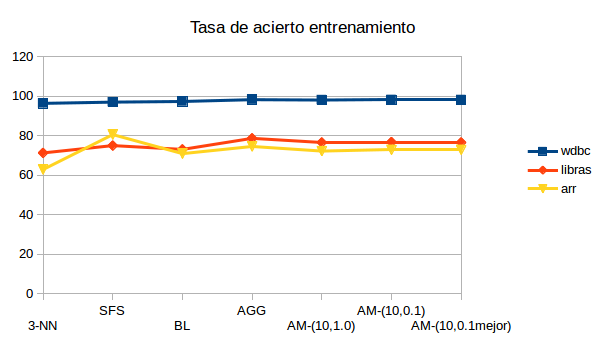
\includegraphics[width=130mm]{tasa_train_am.png}
\end{figure}

Como podemos ver la tasa de acierto sobre Wdbc es la más elevada con respecto a las otras bases, además las tasas de acierto de todos lo algoritmos sobre esta base son muy parecidas, esto se debe a que, como dijo el profesor, esta base de datos es muy pequeña, es decir, el espacio de búsqueda es muy pequeño ($2^{30}$) y hay muy poca tasa de mejora entre una solución y otra.\\

Las tasas de acierto tanto para arritmia como para libras no difieren más que aproximadamente un 5\% para cada algoritmo (excepto para KNN). Es importante señalar cómo la tasa de acierto de los algoritmos usados en mejor que la tasa que da el 3NN original, es decir, usando todos los datos de la muestra. Con lo cual aquí se pone de manifiesto cómo el hecho de reducir el número de características a considerar no merma la correcta clasificación de los datos, al menos dentro de la muestra, ya veremos qué sucede fuera. De hecho reduciendo el número de características no sólo reducimos el cómputo necesario sino también el posible ruido que puedan aportar todos los datos.\\

Es curioso ver cómo el algoritmo greedy produce los mejores resultados en la base de datos con un espacio de búsqueda mayor, de hecho produce mejores resultados en esa base de datos que en la de libras que tiene un espacio menor (es el único que lo hace), probablemente por la naturaleza de los datos, es decir, cómo de distintas sean las muestras que componen las distintas clases entre sí. En mi opinión el hecho de que el SFS produzca mejores resultados que la mayoría en el espacio de búsqueda más grande se debe a que al fin y al cabo el greedy en cada momento va construyendo la mejor solución que puede mientras que en cambio el resto de métodos depende más de cómo de buena sea la exploración que realicen.\\

En cambio sí podemos ver cómo para el espacio más reducido de libras (también se ve en wdbc) sí que los algoritmos que hacen una búsqueda más extensa en el terreno, los meméticos y el AGG, dan resultados mejores que SFS ya que exploran más soluciones y por lo tanto tienen mayor posibilidad de encontrar una mejor.\\

Observamos que los algoritmos meméticos sí que mejoran a la BL, es decir, que la capacidad de exploración que tienen hace que se encuentren mejores soluciones que simplemente con la estrategia de explotación de la BL. Ahora bien, algo que me ha sorprendido es que el AGG básico funciona mejor que los meméticos, es decir, la componente de explotación que tienen no es suficiente. También hemos de tener en cuenta que mientras que en los meméticos estamos empleando un tamaño de población de 10 en los genéticos utilizábamos un tamaño de 30 con lo que la diversidad de la búsqueda es mucho mayor, en estos meméticos con un tamaño tan pequeño la convergencia (si además le sumamos la explotación de la BL de baja intensidad) a una zona del espacio debería ser más rápida que en el AGG y por tanto quizás no sean tan buenos exploradores del espacio de búsqueda. Esto se pone algo más de manifiesto si comparamos los tres algoritmos meméticos entre sí, y es que en todas las bases de datos el que peor funciona es el AM-(10,1.0), el que más explotación realiza. Ahora bien, hemos de decir que el rendimiento de los tres meméticos es muy parecido, probablemente debido al reducido tamaño de la población que hace que la explotación no varie mucho entre unos y otros.\\

Es curioso también observar que, pese a que no podemos extraer conclusiones muy importantes al ser el rendimiento de los algoritos tan parecidos, el memético aleatorio funciona mejor que el que aplica optimización sólo al mejor en las bases de datos más pequeñas (y a la inversa en arritmia), estoy podría indicar que la diversidad que ya aportar el genético es suficiente para arritmia y que es importante explotar buenas zonas del espacio de búsqueda, debido a que el espacio es muy grande movernos aleatoriamente puede llevarnos a soluciones mucho peores.\\


\begin{figure}[H]
\centering
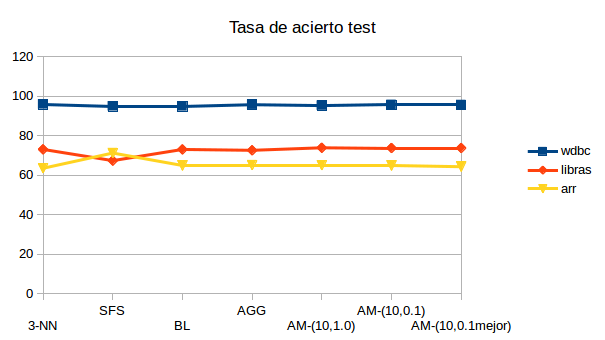
\includegraphics[width=130mm]{tasa_test_am.png}
\end{figure}

Veamos ahora cómo se comportan los algoritmos con respecto a la clasificación que producen sus características seleccionadas para los datos fuera de la muestra de entrenamiento. Lo primero que señalamos es que en la amplia mayoría de los casos la tasa de acierto es mayor dentro de la muestra que fuera, pero hay algunos casos donde es al revés. Esto se debe a que es probable que haya muestras de entrenamiento de una clase más cercanas a otra muestra pese a no pertenecer a la clase de dicha muestra. Con lo cual se puede dar el caso de que la "votación" sea mala en la muestra y en cambio la muestra fuera la distribución de puntos sea más favorable a una correcta clasificación de los datos. Por lo tanto no tiene que extrañarnos demasiado esto. Quizás si usásemos un 1NN sí que sería más probable que la muestra más cercana a otra perteneciera a la misma clase que ella (decimos la más cercana y no que en el 1NN hubiésemos obtenido una tasa de acierto del 100\% dentro de la muestra puesto que usamos para evitar esto el Leave One Out).\\

Nuevamente el comportamiento para Wdbc es muy similar para todos los algoritmos, lo que era esperable por el razonamiento que hemos dado antes. Lo que sí podemos ver es cómo en esta ocasión el 3NN está el primero en wdbc además de que hay otros algoritmos que también cambian de posición. Esto nos informa de dos cosas: la primera es del eterno problema que hay en el aprendizaje automático y es la capacidad de generalización, el no poder asegurar que si una solución es buena dentro de la muestra de entrenamiento vaya a serlo fuera. En segundo lugar vemos cómo lo algoritmos son fuertemente dependientes de los datos, el ruido o simplemente los datos tomados afectan al rendimiento de las soluciones encontradas.\\

El hecho de que el 3NN con toda la información no mejore a todos los algoritmos puede venir de que no sólo haya características irrelevantes sino que, como hemos señalado anteriormente, haya datos cuya medición haya sido errónea y que simplemente lo que nos estén haciendo sea empeorar el resultado.\\

Vemos como en la base de datos menor aquellas estrategias que son más exploratorias son las que funcionan mejor, es decir, que el hecho de tomar la mejor solución (dentro de los límites de la exploración claro) de todo el espacio de búsqueda nos da una buena solución en el test, que la generalización es buena. No obstante en la base de datos de mayor tamaño es el SFS algoritmo sin ninguna exploración el que mejor funcionan, tenemos un espacio de búsqueda tan grande y con tantos datos tan diverso que, el hecho de explorar y buscar la mejor solución para estos datos hace que la generalización sea peor.\\

Aunque nuevamente no podemos extraer unas conclusiones demasiado buenas debido a que el rendimiento de los meméticos es muy parecido vamos a compararlos entre sí: en relación a lo que hemos dicho antes, el memético aleatorio, el que aporta mayor diversidad, es que que peor funciona el las bases de datos mayores y sin embargo el que mejor funciona en wdbc.\\

En la base de libras, que es en la que hemos venido observando un comportamiento algo más sorprendente de los algoritmos desarrollados a lo largo de las prácticas son los algoritmo meméticos lo que mejor funcionan, es decir, es una base de datos tan "extraña" que el equilibrio exploración-explotación que aportan estas estrategias es la que mejor se adapta.\\

\begin{figure}[H]
\centering
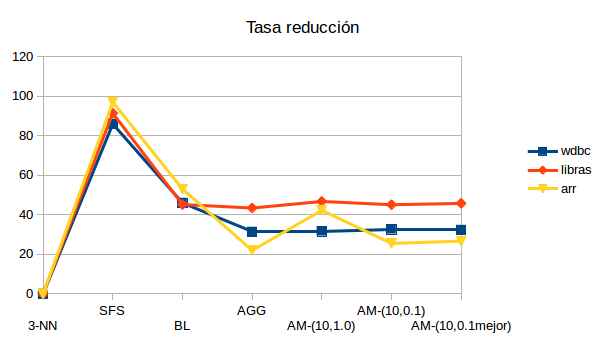
\includegraphics[width=130mm]{reduccion_am.png}
\end{figure}

Evidentemente la tasa de reducción para el 3NN es 0 pues tomamos todas las características al no tener otro criterio. Ahora el que produce mayor reducción es el greedy lo que es lógico por la forma en la que trabaja, agregando progresivamente propiedades hasta no encontrar mejora ninguna.\\

El siguiente algoritmo que menos reduce es el AGG que es el más exploratorio seguido del siguiente más exploratorio que es el memético aleatorio, (10, 0.1), con lo cual como vemos cuando los algoritmos son más explotativos tienden a seleccionar un mayor número de características, aquí puede verse la tendencia al sobreajuste, al querer adaptarse a estos datos toma la información como relevante y por tanto no la descarta ya que obtiene mejores tasas de clasificación con toda la información.\\

Esto lo podemos ver en arritmia donde el orden de los algoritmos de mayor a menos tasa de reducción es exactamente el mismo que de mayor a menor explotación: SFS, BL, AM-(10,1.0), AM-(10,0.1mejor), AM-(10,0.1), AGG y 3NN.\\

En las bases de datos de libras y wdbc no se observa esto tan claramente pero también es cierto que hay menos variación entre las distintas tasas de reducción de los algoritmos en estas bases.\\

\begin{figure}[H]
\centering
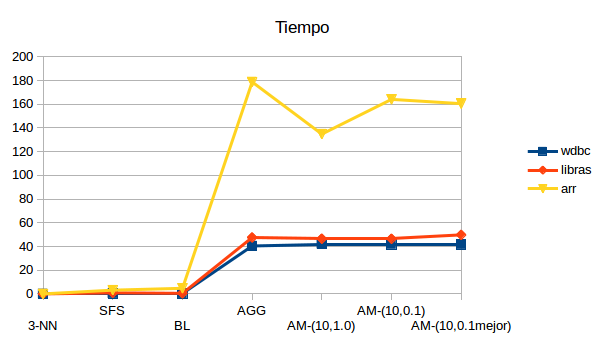
\includegraphics[width=130mm]{tiempo_am.png}
\end{figure}


Evidentemente el 3NN tarda 0 segundo puesto que su tiempo de búsqueda de solución es 0 pues simplemente devuelve un solución con todos los valores a True, es decir, escoge todas las características sin tener ningún criterio. Y observamos también que todos los algoritmos si los analizamos individualmente tardan más cuanto mayor es el espacio de búsqueda (ahora el LOO no tiene tanto impacto y con lo cual el número de muestras por partición no resulta tan decisivo como sí ocurría en la primera práctica cuando se tardaba más en libras que en arritmia para algunos algoritmos).\\

Los algoritmos que menos tardan son BL y SFS lo cuál es lógico ya que dependen simplemente de cómo de rápido converjan, como vemos la convergencia de BL es mś rápida en las bases de datos de menor tamaño con lo que la hay diversidad en la base de datos de mayor tamaño.\\

En las bases de datos de menor tamaño las diferencias de tiempo entre los distintos meméticos y el AGG no son muy grandes es decir la BL de baja intensidad no aporta demasiada carga en tiempo de cómputo ya que es en un espacio pequeño.\\

En la base de datos de arritmia, donde la BL de baja intensidad puede ser más lenta ya que el vecindario de un inviduo es mayor, sí vemos como el AGG es más rápido al no realizar BL que los meméticos. Además entre los meméticos el más lento en esta base es el que aplica más búsquedas locales, el AM-(10,1.0) y en cambio los otros dos que realizan el mismo número de BL (ya que el tamaño de la población es 10) tarda prácticamente lo mismo.\\

\newpage
\section{\color[rgb]{0.0,0.0,0.21}Bibliografía}

\begin{itemize}
\item Documentación del módulo scikit-learn: \url{http://scikit-learn.org/stable/documentation.html}
\item Documentación de Numpy: \url{http://docs.scipy.org/doc/}
\end{itemize}
\end{document}